\addcontentsline{toc}{chapter}{Transport Layer}
\chapter*{\begin{center}Transport Layer\end{center}}
\begin{center}(Layer 4 nello stack TCP/IP)\end{center}\hrulefill \\
\noindent A livello di trasport, Internet utilizza due protocolli\footnote{nota: sebbene TCP e UDP siano i due protocolli più diffuso per il transport layer, non sono gli unici due protocolli esistenti per il trasporto in assoluto!}
\begin{itemize}
    \item TCP;
    \item UDP;
\end{itemize}
\noindent Sappiamo già che TCP è connection-oriented, con meccanismi di controllo della congestione e di flusso e di sicurezza etc., laddove invece UDP si limita a spedire il pacchetto dove gli viene indicato e Dio provvede di quello che succede al pacchetto.\\

\noindent Un pacchetto dati a livello di trasporto prende il nome di \underline{segmento:}\index{segmento} in alcuni documenti e RFC\footnote{non li avevo menzionati finora? RFC sta per Request For Comment, sono documenti che stabiliscono praticamente degli standard di questo e quel protocollo o meccanismo, li pubblicano svariati enti come la IETF.}, i segmenti vengono chiamati anche \openapex datagram'', ma con quel termine c'è un piccolo problema di ambiguità: infatti, con il termine \openapex datagram'' ci si riferisce anche ai pacchetti dati che raggiungono il livello di rete. Tutte le mie source utilizzano il termine \openapex segmento'', quindi magari usiamo quello e basta.\\

\noindent In genere, un segmento a livello di trasporto contiene tre elementi:
\begin{enumerate}
    \item nr. porta di origine / nr. porta di destinazione (campi lunghi 16 bits ciascuno, per un totale di $16+16=32$);
    \item altri campi di intestazione\footnote{useremo i termini \openapex intestazione'' e \openapex header'' intercambiabilmente.} (tipo e lunghezza variano tra TCP e UDP); 
    \item messaggio (il contenuto).
\end{enumerate}

\begin{figure} [h]
    \centering
    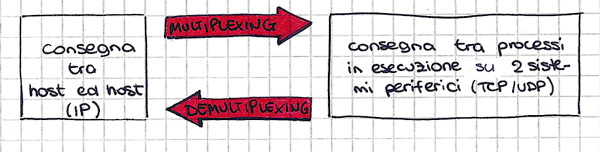
\includegraphics[width=0.75\linewidth]{Figures/03/mpx-dmpx.png}
\end{figure}


\noindent Multiplexing\index{multiplexing} a livello di trasporto: raduna diversi dati da diverse socket e li incapsula in un unico pacco di dati da spedire in rete (è importante che ogni socket abbia un numero di porta per completare questa operazione in avanti e indietro). In genere multiplexing è una qualche operazione che prende n input ed ha 1 output;\\

\noindent Demultiplexing\index{demultiplexing} a livello di trasporto: esamina determinati campi del messaggio ricevuto e decide a quale socket del ricevente consegnarlo. Qui stiamo parlando di ricevere da un unico input e di distribuire il contenuto ricevuto a n possibili output;\\

\noindent Sia TCP che UDP fanno MPXing e DMPXing.\\

\noindent \textit{Nota abbastanza importante sui numeri di porta\index{porta!numeri di}\index{porte!note}\index{porte!effimere}\index{porte!private}:
\begin{itemize}
    \item le porte numerate da $0\div1023$ vengono dette \openapex porte note'' perché sono riservate a servizi quali HTTP. Non si possono usare arbitrariamente per altre cose;
    \item le porte comprese tra $1024\div49552$ si chiamano \openapex indirizzi effimeri'', assegnati randomicamente al momento dell'apertura della porta;
    \item le porte comprese tra $49553\div65535$ sono \openapex porte private''.
\end{itemize}}
%%%%%%%%%%%%%%%%%%%%%%%%%%%%%%%%%%%%%%%%%%%%%%%%%%%%%%%%%%%%%%%%%
\addcontentsline{toc}{section}{UDP}
\section*{UDP}
\underline{U}ser \underline{D}atagram \underline{P}rotocol\index{UDP}
\begin{itemize}
    \item Protocollo connectionless - niente handshake a inizio connessione. Questo riduce notevolmente la congestione e rende così UDP per certi versi più veloce di TCP;
    \item \openapex senza fronzoli'': l'intestazione di un pacchetto UDP è lunga solo 8 Byte (contro quella di TCP che è lunga ben 20)
\end{itemize}

\noindent Header (intestazione) segmento UDP:
\index{UDP!header}
\begin{table}[h]
\begin{tabular}{cc}
\textit{(2 Bytes)}                                                               & \textit{(2 Bytes)}                                                                       \\ \hline
\multicolumn{1}{|c|}{\begin{tabular}[c]{@{}c@{}}Porta di\\ origine\end{tabular}} & \multicolumn{1}{c|}{\begin{tabular}[c]{@{}c@{}}Porta di\\ destinazione$^1$\end{tabular}} \\ \hline
\multicolumn{1}{|c|}{Lunghezza msg$^2$}                                          & \multicolumn{1}{c|}{checksum$^3$}                                                        \\ \hline
\end{tabular}
\end{table}
\noindent $^1$: usata per Demultiplexing;\\
$^2$: indica dove finisce il messaggio;\\
$^3$: per verificare errori nel messaggio: se i complementi a 1 sono andati a buon fine (e quindi anche l'invio/ricezione del pacchetto), il risultato del checksum deve essere uguale a $11111111$ $11111111$ (16 volte 1).\\
\index{checksum}
\noindent UDP non fa niente che non sia Multiplexing e Demultiplexing. Per la maggior parte dei protocolli dell'application layer (tipo HTTP) viene utilizzato TCP, perché TCP fornisce molti servizi legati alla stabilità e affidabilità della connessione. UDP viene usato perlopiù dove è richiesta non tanto correttezza di tutti i pacchetti ma piuttosto una alta responsiveness (quindi tempi d'attesa brevissimi) e ci si può permettere una certa percentuale di packet loss senza influire sul risultato visibile in maniera critica - quindi in servizi come streaming video o VoIP (voice over IP, ossia Skype, Discord etc., ma viste le performance di internet si sta iniziando ad usare TCP anche per questi qui).\\


\addcontentsline{toc}{section}{RTD}
\section*{RDT - Principi di Trasferimento Dati Affidabile}
\index{RDT}
\noindent Piccola digressione in cui parleremo, in maniera un po' teorica, del sistema di trasferimento dati affidabile (\underline{R}eliable \underline{D}ata \underline{T}ransfer, RDT): una serie di meccanismi da adottare per prevenire la perdita di informazione a seconda dei vari problemi che ci possono essere (ritardi, timeout, errori etc.). Questo perché TCP, per quanto premuroso possa essere come protocollo, si appoggia a protocolli a livello sottostante che non sono in grado di garantire davvero una comunicazione perfetta: qualcosa può andare male, e servono strategie per mitigare questo \openapex male''.
\addcontentsline{toc}{subsection}{RDT 1.0}
\subsection*{RDT 1.0 - Canale Affidabile}
\index{RDT!1.0}
\noindent L'approccio naïve, ovvero quello basato sull'assunzione che il canale sottostante sia perfettamente affidabile. Quindi non fa nulla di contromisure. 

\begin{figure} [ht]
    \centering
    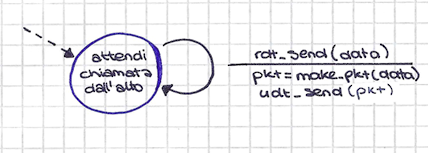
\includegraphics[width=0.8\linewidth]{Figures/03/rdt1-0-mit.png}
    \caption{RDT 1.0, lato mittente. Spieghino veloce di cosa succede qui: c'è uno stato solo, in cui il mittente attende la chiamata dall'alto (ovvero dal layer sopra); quando riceve il comando \openapex send(data)'', risponde con 2 azioni - crea il pacchetto con i dati e le info necessarie, e lo invia.}
\end{figure}

\begin{figure} [h!]
    \centering
    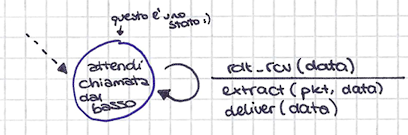
\includegraphics[width=0.8\linewidth]{Figures/03/rdt1-0-rcv.png}
    \caption{RDT 1.0, lato ricevente. Quando viene ricevuta una chiamata \openapex receive(data)'', estrae i dati dal pacchetto (extract) e li consegna al layer sopra (deliver). Come dicevamo, nessuno dei due lati fa nient'altro.}
\end{figure}
\newpage

\addcontentsline{toc}{subsection}{RDT 2.0}
\subsection*{RDT 2.0 - Rilevamento Errori}
\index{RDT!2.0}
\noindent Supponiamo ora che ci possano essere errori. Dobbiamo quindi fare in modo che il lato ricevente dia un feedback (ACK, NAK). Chiamiamo questo approccio error detection-feedback-retransmission.\footnote{La famiglia di protocolli che fanno questo tipo di cosa si chiama ARQ, Automatic Repeat reQuest (o Query).}

\begin{figure} [h]
    \centering
    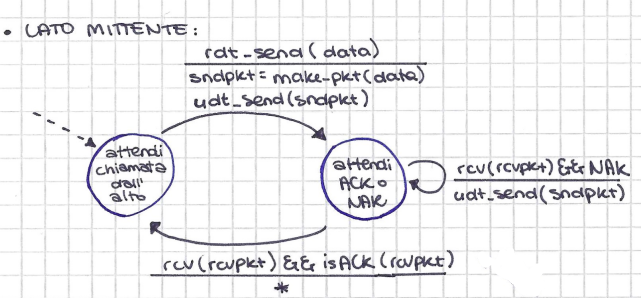
\includegraphics[width=0.75\linewidth]{Figures/03/rdt2-0-snd.png}
    \caption{RDT 2.0, lato mittente. Questo ha 2 stati, uno di attesa chiamata e uno di attesa feedback: RDT riceve la chiamata \openapex send'', quindi impacchetta, spedisce il messaggio e si mette in attesa di feedback. Se arriva un NAK (ovvero errore rilevato), allora rispedisce lo stesso pacchetto di nuovo; altrimenti (ACK), torna in attesa che il layer sopra gli passi un nuovo pacchetto da inviare.}
    \label{fig:rdt2.0s}
\end{figure}

\begin{figure} [h]
    \centering
    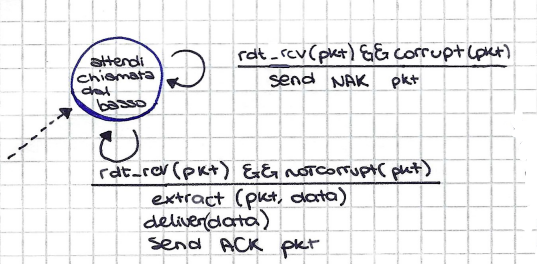
\includegraphics[width=0.6\linewidth]{Figures/03/rdt2-0-rcv.png}
    \caption{RDT 2.0, lato ricevente. Qui, all'arrivo di un messaggio dal layer sottostante, possono succedere 2 cose: il pacchetto non va bene (corrupt) $\rightarrow$ invia NAK in risposta; il pacchetto va bene $\rightarrow$ risponde ACK al mittente e consegna il pacchetto al layer sopra.}
    \label{fig:rdt2.0r}
\end{figure}
\newpage
\noindent Semplice semplice. Ora però sorge un altro problema ancora: e se fosse il pacchetto contenente \openapex ACK/NAK'' ad essere corrotto? $\rightarrow$ soluzione: aggiungere ad ogni pacchetto un nuovo campo di informazione: il Sequence Number\index{sequence number}. Tipicamente vengono usati numeri naturali crescenti, ma è sufficiente anche alternare messaggi con SN 0 e SN 1 perché la magia funzioni.


\bigskip
\addcontentsline{toc}{subsection}{RDT 2.1}
\subsection*{RDT 2.1 - Sequence Numbers}
\index{RDT!2.1}
\begin{figure} [h]
    \centering
    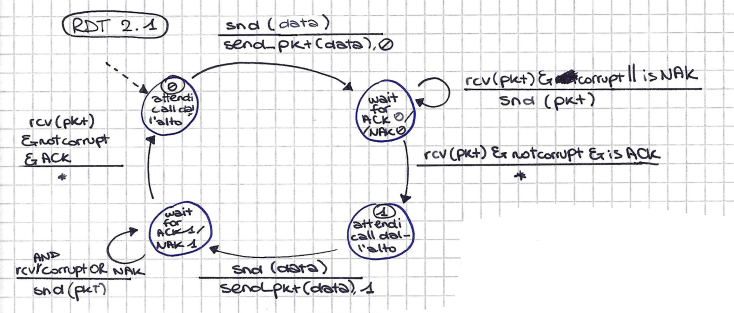
\includegraphics[width=0.7\linewidth]{Figures/03/rdt2-1-s.png}
    \caption{RDT 2.1, lato mittente: questo qui fondamentalmente dice: se il pacchetto di feedback arriva corrotto o contentente un NAK, in base allo stato dell'automa in cui mi trovo o rispedisco il pacchetto con SN = 0 oppure quello con SN = 1; in questa maniera, se il destinatario aveva capito il messaggio con SN 0 e il mittente gli manda un pacchetto con lo stesso SN, il destinatario si rende conto che è una ripetizione e non una nuova trasmissione. (E questo credo sia tutto ciò che cambia lato destinatario, spero sia la ragione per cui ho omesso l'automa del lato destinatario interamente)}
    \label{fig:rdt-21s}
\end{figure}

\newpage
\addcontentsline{toc}{subsection}{RDT 2.2 e RDT 3.0}
\subsection*{RDT 2.2 e 3.0 - ACK duplicati e Time-out}
\index{RDT!2.2}\index{RDT!3.0}\index{ACK!duplicati}\index{time-out}
\noindent In breve, RDT 2.2 introduce al posto di ACK e NAK, soltanto l'uso di ACK ma duplicati, nel senso: invece di mandare un messaggio del tipo \openapex non ho capito questo'' dice \openapex l'ultimo messaggio che ho capito bene è quello'' (identificando \textit{questo e quello} con i sequence number dei messaggi in questione.);\\
\noindent RDT 3.0 introduce il meccanismo di Time-out: è possibile che un pacchetto si smarrisca per strada, quindi si fa uso di una sorta di countdown per ogni pacchetto - un timer, se vogliamo - per stabilire se e quando smettere di aspettare un riscontro.\\
\noindent Credo e spero che non valga la pena annettere gli automi che illustrano il funzionamento anche di questi due, perché sono sempre più densi di stati e comportamento che trovo più facile riassumere a parole. È una scelta che invecchierà male? Lo scopriremo (ma non credo).\\

\noindent E questi sono protocolli di tipo \openapex Stop-and-Wait''\index{protocollo!stop-and-wait} che approcciano il problema della gestione degli errori tramite attesa di feedback o time-out; ora vedremo il GO-BACK-N, che è una famiglia di protocolli che ha a che fare con il \openapex pipelining''\index{pipelining} - ovvero, invece di fermarsi ad aspettare feedback ogni volta che si manda un singolo pacchetto, se ne mandano $n$ uno dietro l'altro. È indubbiamente più efficiente, ma quanti pacchetti posso mandare in sicurezza senza che un errore a un certo punto generi fatalmente \textit{chaos \& confusion}?

\addcontentsline{toc}{subsection}{Go-Back-N}
\subsection*{Go-Back-N}
\index{Go-Back-N}
\noindent Per rispondere alla domanda di cui sopra, si fa uso di quella che viene chiamata \index{finestra scorrevole}\openapex finestra scorrevole''\footnote{da non confondere con la finestra di congestione, meccanismo di controllo congestione TCP (TCP Reno).}: la larghezza di questa finestra cambia dinamicamente ma non a caso, la dimensione della finestra viene adattata dal controllo di flow e congestione!\index{congestione}

\begin{figure} [h]
    \centering
    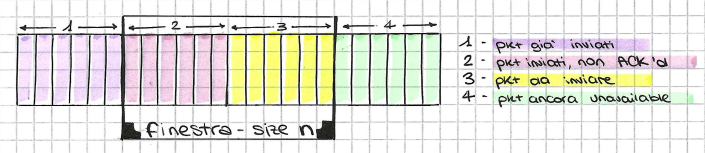
\includegraphics[width=1\linewidth]{Figures//03/window.png}
    \caption{Quanto mi piace usare 'sti colori. Finestra scorrevole, con annessa adorabile legenda dei colori. L'ultima parola a destra nel punto 4 è \openapex unavailable'', ndr.}
    \label{fig:congwin}
\end{figure}

\noindent Riscontro cumulativo\index{riscontro cumulativo}: mandare un ACK per il pacchetto numero N implica che tutti i messaggi fino ad N sono stati ricevuti correttamente $\approx$ \openapex fino a N li ho capiti tutti''. In caso di time-out, il mittente rispedisce tutti i pacchetti della zona 2 (in rosa\footnote{pastello! :D}), cioè quelli inviati ma non confermati da ACK.\\
\noindent Selective Repeat (SR)\index{selective repeat}: \openapex non ritrasmettere tutto quanto, ma solo le parti che non ho capito'' (starà poi al ricevente metterli nel giusto ordine quando vengono ritrasmessi e ricevuti).

\addcontentsline{toc}{section}{TCP}
\section*{TCP}
\index{TCP}
\underline{T}ransmission \underline{C}ontrol \underline{P}rotocol\\

\epigraph{With TCP, two hosts are a company, and three are a crowd.}{\textit{Una qualche edizione del Kurose-Ross}}

\begin{itemize}
    \item connection-oriented: prevede che si faccia un handshake (lit. \openapex stretta di mano'') prima di iniziare lo scambio di messaggi vero e proprio;
    \item sempre point-to-point: connette un solo host con un solo host, fine.
\end{itemize}

\noindent Fantastici parametri TCP e a quali sigle trovarli:
\index{TCP!parametri}
\begin{itemize}
    \item \index{MSS}MSS, Maximum Segment Size: limite di dati che possono essere messi in un segmento TCP. Questo parametro dipende dal (vedi punto successivo)
    \item \index{MTU}MTU, Maximum Transmission Unit: dimensione massima dei dati che possono essere gestiti al livello datalink - ad esempio, Ethernet ha una MTU di 1500 Bytes;
    \item \index{TCP!flag}Flag TCP! Da ricordare. Sono bit (quindi valori di lunghezza 1 che possono essere o $=0$ o $=1$). Vediamole:
    \begin{itemize}
        \item RST: sta per \openapex ReSeT'', si usa in caso di gravi errori;
        \item PSH: (PUSH, credo) indica al ricevente di passare subito questo segmento al layer soprastante, senza elaborare niente;
        \item URG: manca il contenuto del segmento come URGente;
        \item FIN e SYN: si usano rispettivamente per indicare una chiusura e un'apertura della connessione; 
        \item ISN: Initial Sequence Number: numero generato in modo pseudorandomico all'avvio di una connessione TCP. È compreso tra i valori $0\div(2^{32}-1)$, da quel numero in poi si conteranno i sequence number (tipicamente in modo crescente, andando di successori);
        \item MSL: Max Segment Lifetime, il tempo durante il cui il segmento resterà in vita nella rete. Scaduto questo tempo, il pacchetto viene soppresso;
        \item CWR e ECE, le vedremo più avanti.
    \end{itemize}
    Queste flag appaiono nel header TCP nel seguente ordine: CWR - ECE - URG - ACK - PSH - RST - SYN - FIN;
\end{itemize}

\noindent Fattore di Time-out: ci interessa che il Time-out sia maggiore del RTT (round-trip time), naturalmente, altrimenti il pacchetto non ha nemmeno modo di arrivare a destinazione perché muore prima. In TCP, il RTT viene preso ad ogni ACK. Non può essere stabilito a priori, al limite si può stimare.\\

\noindent estimatedRTT:
\[eRTT = (1-\alpha)\cdot eRTT + \alpha \cdot sampleRTT\]
\noindent $\alpha$ è un fattore costante, di solito $=0,125$, per fare una media pesata di quei due parametri; $sampleRTT$ è il RTT misurato \textit{(sampled)} per ogni andata e ritorno.\\

\[devRTT = (1-\beta)\cdot devRTT + \beta \cdot (sampleRTT - eRTT)\]
\noindent con $\beta = 0,25$, questa è la deviazione standard RTT. Alla fine, il RTT calcolato avrà valori che convergono in modo abbastanza stabile, e la deviazione standard valori abbastanza bassi.\\

\noindent Notine di dubbia utilità di lab:
\begin{itemize}
    \item TSHARK non è altro che Wireshark ma con una interfaccia command line anziché interfaccia grafica;
    \item Wireshark ha un tool per l'analisi RTT: \begin{verbatim}
        tcp.analysis.ack_rtt
    \end{verbatim}
\end{itemize}

\noindent \index{RTO}RTO: Retransmission Time-Out: tempo entro cui la sorgente si aspetta di ricevere un riscontro. Non può essere un valore statico predefinito, dipende da moltissimi fattori. Si calcola dinamicamente (perché basato sul RTT, che si calcola dinamicamente), di solito il risultato è compreso tra $200ms<RTO<60+sec$:
\[RTO = eRTT + 4 \cdot devRTT\]

\noindent \index{window!receive}RcvWindow: Buffer che serve ad evitare problemi di flusso dei dati. Memorizza i byte ricevuti per poi passarli all'app layer. Quando questo buffer è pieno, il destinatario manda byte di controllo al sender per dire che non può ricevere nient'altro al momento. Appena si liberano $n$ bytes, il destinatario\footnote{probabilmente per abitudine tenderò ad abbreviare mittente e destinatario con snd e rcv qualche volta (sender, receiver), sapevatelo} invia un messaggio al mittente per dire \openapex Ok, ora ho spazio, mi aspetto messaggi a partire da $<$(ultimo messaggio ricevuto $+1>$ e ho $n$ byte di spazio.''
\newpage
\addcontentsline{toc}{subsection}{Handshake TCP}
\subsection*{\textcolor{blue}{SYN-SYNACK-ACK, il Three-Way Handshake in TCP}}
\noindent \index{handshake!three-way}\index{TCP!handshake}È un concetto abbastanza importante. Fondamentalmente questo è ciò che va fatto prima di avviare ogni conversazione tra host TCP. È come quando al telefono ci si risponde \openapex Pronto, chi è?'' \openapex Sono Tizio, tu sei Caio?'' \openapex Ciao Tizio, sì io sono Caio''. Una fase di autenticazione preliminare, insomma. Fatto questo, si può iniziare la conversazione vera e propria.\\

\begin{figure} [h]
    \centering
    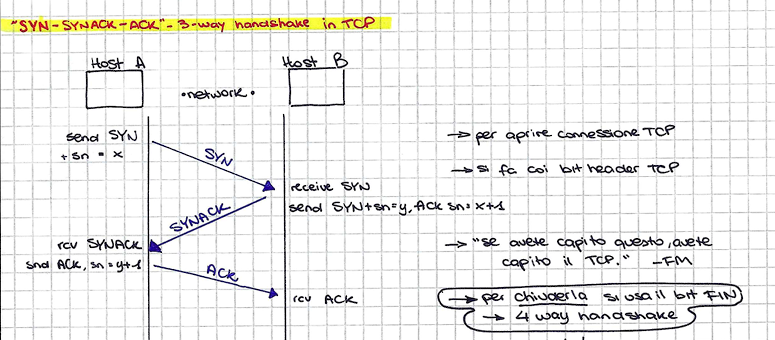
\includegraphics[width=1\linewidth]{Figures/03/tcp-3whs.png}
    \caption{Three-way handshake TCP.}
    \label{fig:3whsTCP}
\end{figure}

\noindent Finita la conversazione, per continuare la metafora della telefonata, vogliamo segnalare che abbiamo finito di parlare, quindi dire una cosa come \noindent Va bene, ora ti saluto, ciao!'', a cui l'interlocutore risponde \noindent OK, ciao!'' e poi si riattacca. Paradossalmente questo si fa in 4 messaggi, più di quanti non ce ne vogliano per iniziare la conversazione - ma queste sono le meraviglie di TCP. Comunque, \index{handshake!four-way}4-way handshake di chiusura in Fig. \ref{fig:4whsTCP}:

\begin{figure} [h]
    \centering
    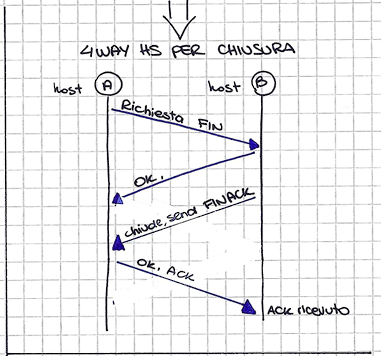
\includegraphics[width=0.5\linewidth]{Figures/03/4whstcp.png}
    \caption{Handshake di chiusura TCP.}
    \label{fig:4whsTCP}
\end{figure}

\noindent Controllo della congestione, nota: immettere in rete dei \openapex pacchetti di controllo'' a scopo di controllo della congestione è fortemente sconsigliato, paradossalmente congestiona esso stesso la rete.\\

\noindent Il discorso su prestazioni e scenari relativi è discusso in maniera molto esaustiva sia nel libro che nelle slides, you're on your own with this one $>:)$\\

\noindent Comunque ci sono due approcci principali al \index{controllo congestione}congestion control: End-to-End e Network-assisted. Per quanto riguarda TCP e il congestion control, occorre parlare di finestra di congestione\index{finestra di congestione}.\\
\noindent congWindow: finestra di congestione. Quantità di dati riscontrati da un host durante la connessione. Vincolo: TCP non può inviare dati ad un rate maggiore della ampiezza della finestra di congestione, e questa finestra, come ha senso che sia, cambia ampiezza dinamicamente a seconda del livello corrente di congestione. Per cambiare il ritmo di invio in funzione della congestione si usano diversi approcci (io qui li ho chiamati Algoritmi, non so se sia accurato come termine, ma penso stessi facendo riferimento ai TCP Tahoe e Reno)\index{TCP!Tahoe}\index{TCP!Reno}:
    \begin{itemize}
        \item AIMD: incremento additivo, decremento moltiplicativo;
        \item Slow Start: per ogni ACK ricevuto, raddoppio la dim. della finestra;
        \item Fast Recovery: questo non lo vedremo, rip
    \end{itemize}
\noindent Threshold (soglia): limite tra decremento moltiplicativo e incremento additivo: se il valore corrente è $<Thr \rightarrow$ si adotta slow start; se il valore corrente è $>Thr\rightarrow$ si adotta congestion avoidance (AIMD). Nel modulo di tutorato si vedono meglio questi discorsi con TCP Reno e compangia. Comunque, l'idea è che l'algoritmo vada a convergere e stabilizzarsi su un certo range di rata di trasmissione, anche se nella pratica poi non va così (vedasi TCP CUBIC, non ho nessuna memoria di cosa sia questa roba).\\

\addcontentsline{toc}{subsection}{Note di Lab}
\subsection*{\textcolor{RoyalPurple}{Note di Lab:}}
Nmap, network scanner! 2 tecniche principali:\index{nmap}
\begin{itemize}
    \item PORTSCAN\index{port!scanning}: attività promiscua (losca, sospetta), da usare solo previa autorizzazione se non vogliamo cacciarci in qualche guaio, perché il port scanning di solito è una tecnica utilizzata per scoprire porte aperte in altri dispositivi, al fine di sfruttarne le vulnerabilità e provare qualche attacco. Port scanning aiuta un malintenzionato a trovare porte aperte e a capire se queste sono in ascolto o stanno trasmettendo dati. Inoltre, può rivelare misure di sicurezza (come un firewall) sono in uso in qualche rete aziendale\footnote{ fonte \href{https://www.fortinet.com/resources/cyberglossary/what-is-port-scan}{Qui}};
    \item PING SWEEP\index{ping!sweep}: port monitoring, analisi di sicurezza, information gathering, attacchi, beh suona abbastanza simile al port scanning. Il ping sweeping consiste in mandare messaggi di ping a più indirizzi IP per trovare degli host \openapex vivi'' (insomma accesi) nella rete, da cui poi si procede col port scanning sugli host vivi.\footnote{Se volete divertirvi a leggere/guardare, ho trovato \href{https://study.com/academy/lesson/ping-sweeps-definition-tools-uses.html}{questo}}
\end{itemize}
\texttt{nmap} utilizza delle \openapex fingerprints'' (impronte digitali) per raccogliere informazioni su di un target. Eventualmente è possibile utilizzarlo con interfaccia grafica (che si chiama Zenmap), ma \textit{il prof, con un velo di sarcasmo, ci fa sapere che \openapex Zenmap è per quegli utenti che usano il Mac''.} Nmap ha incorporato uno script engine in LUA, ovvero una collezione di script che si possono eseguire per trovare vulnerabilità e affini. Basta eseguire il comando \begin{verbatim}
    nmap --script-updatedb
\end{verbatim}
per aggiornare questa fantastica lista di script curata dagli eroi invisibili della rete.\\
\noindent ncat invece è un tool open source a riga di comando utile a collegarsi ad un altro host da remoto, pretty cool. Tutte le info che abbiamo visto di ncat si trovano nelle slides del prof - a \href{https://computerscience.unicam.it/marcantoni/}{questo indirizzo}, nella tabella \openapex didattica'' $>$ Internet, Reti e Sicurezza $>$ Esercitazioni e Laboratorio Wireshark al nome \openapex nmap.pdf''.